\section{Physics-Derived Detectability, Forgetting and Integrity}
\label{sec:theory}

Each retained history is linear-Gaussian given its mode path. The
information that the eight PMUs carry about every candidate intervention
can therefore be computed from the predictor operators before any
attribution experiment is run. This section derives these quantities,
extends them to missing and corrupted PMUs and states what they predict;
Sections~\ref{sec:narrative-results}, \ref{sec:noise-stress}
and~\ref{sec:integrity-results} test the predictions.

\subsection{Signatures and Information}
Let intervention $i$ start at report $0$ with severity $a$ and let the
plant follow the local switched model \eqref{eq:implemented-predictor}
without noise. Run the conditional filter of candidate history $j$, started
at the same onset, on these reports. Its innovation $e_j(k)$ and severity
sensitivity $s_j(k)$ follow the recursion
\eqref{eq:implemented-conditional-correction}. The filter of the true
history at the true severity has zero innovation, so the expected
log-likelihood ratio of $i$ against $j$ after $k$ reports is the
whitened signature energy
\begin{equation}
 \Lambda_{ij}(k)=\tfrac12\min_{b\in[l,u]}\sum_{r=0}^{k}
 \big\|e_j(r)-s_j(r)\,b\big\|^2_{S_j^{-1}},
 \label{eq:signature-information}
\end{equation}
where the minimization over the competitor's severity is omitted when $j$
is a line. With $j$ the no-intervention history, $\Lambda_{i0}$ is the
\emph{detection information}; $\min_{j\neq i}\Lambda_{ij}$ is the
\emph{isolation information}. Both follow from the reduced input
directions, the topology offsets $c_q$ and $d_q^{\rm el}$, the terminal map
and the instrument model; no data are fitted. For a load,
$\Lambda_{i0}=\tfrac12a^2G_i(k)$, with $G_i$ the accumulated information
per unit severity squared. In change detection--isolation theory the
asymptotic delay at a fixed error level is inversely proportional to this
information rate \cite{lai2000sequential,tartakovsky2014sequential}.

With birth prior $\pi_c$ per report and cell, the active mass of the true
history at its own onset reaches $0.99$ once
\begin{equation}
 \Lambda_{i0}(k)\ \ge\ \lambda^\star=\log 99-\log\pi_c,
 \label{eq:alarm-evidence}
\end{equation}
which is $\lambda^\star\approx\RevInfoNeed$ nats for the configuration of
Section~\ref{sec:narrative-method}. The minimum load change detectable
within a horizon $T$ under a noise standard-deviation multiplier $\alpha$
is then
\begin{equation}
 a_{\min}(\alpha,T)=\alpha\sqrt{2\lambda^\star/G_i(T)}.
 \label{eq:minimum-detectable}
\end{equation}

\subsection{The Cost of Forgetting the Physical State}
Suppose the conditional mean tracks the augmented state until an inferred
closure at report $k_c$. If the state is carried, the innovations after
$k_c$ keep zero mean. If the physical coordinates are set to zero while
the instrument and discrepancy states are kept, the no-intervention filter
receives the deterministic bias
\begin{equation}
 \bar e_0(k)=C_0\Phi_0(k,k_c)\,\delta x(k_c)
 -\!\!\sum_{r=k_c}^{k-1}\!C_0\Phi_0(k,r{+}1)K_0\,\bar e_0(r),
 \label{eq:reset-bias}
\end{equation}
where $\delta x(k_c)$ is the zeroed physical part of the augmented state,
$\Phi_0(k,r)=T_0^{\,k-r}$ and $C_0=J_0$ are the no-intervention operators of
\eqref{eq:implemented-conditional-correction}, and $K_0$ is its gain. This
is the free recovery response \eqref{eq:recovery-response} seen through a
filter that tries to absorb it. Any birth hypothesis $j$ that explains part
of this bias gains
$\Gamma^{\rm sp}_j(k)=\Lambda^{\rm reset}_{0}(k)-\Lambda^{\rm reset}_{j}(k)$
over the no-intervention history, and a spurious alarm becomes possible
when $\max_{j,k}\Gamma^{\rm sp}_j(k)\ge\lambda^\star$. With carry,
$\Gamma^{\rm sp}_j\equiv0$. The bias, and therefore the cost of forgetting,
grows with the energy of the slow electromechanical modes excited by the
intervention and with how strongly the PMUs observe them.

\subsection{Measurement Integrity}
\label{sec:integrity-theory}
The competition data also contain integrity events: frames that never
arrive and frames whose values are corrupted. Write the received report of
PMU $p$ as
\begin{equation}
 y_{p,k}=M_{p,k}\big(h_p(x_k)+v_{p,k}+\beta_{p,k}\big),
 \label{eq:integrity-observation}
\end{equation}
where $M_{p,k}\in\{0,1\}$ is availability and $\beta_{p,k}$ a corruption
that does not enter the network equations. Availability is observed through
the frame flag, so a missing PMU is identified exactly. What it removes is
information, and the same quantity governs corruption.

\begin{proposition}[Integrity isolation]\label{prop:integrity}
Let the noise be Gaussian and independent across PMUs, and let the
corruption of PMU $p$ be unrestricted over a window. The generalized
likelihood ratio that separates physical source $i$ from ``no
intervention, PMU $p$ corrupted'' carries the information
$\Lambda_{i0}^{(-p)}$, the detection information of $i$ computed without the
channels of PMU $p$. This is also the information for $i$ when PMU $p$ is
missing.
\end{proposition}
\emph{Proof.} Profiling an unrestricted $\beta_p$ projects the signature onto
the orthogonal complement of the channels of PMU $p$. With block-diagonal
noise covariance this projection deletes those channels, and the remaining
quadratic form is the information of the other PMUs. \hfill$\square$

With cross-PMU noise correlation, deletion is replaced by the Schur
complement and $\Lambda^{(-p)}$ becomes a conditional information. The
proposition explains why integrity cannot be recognized from a single PMU
alone: a corruption becomes distinguishable only through relations that
every physical event of the network obeys. Two such relations are used.
\emph{Sequence parity.} For balanced interventions (load, line,
generation, three-phase fault) the balanced network produces no negative-
or zero-sequence voltage or current. These sequence components are
therefore parity relations in the sense of analytical redundancy
\cite{chow1984analytical}: they are insensitive to every physical
intervention and sensitive to corruption of a single phase. A step
$\epsilon$ in one phase magnitude gives $|X_2|=|X_0|=\epsilon|X|/3$. The
corrupted phase is the one whose phasor is most aligned with $X_0$.
Under independent per-phase noise, $q_k=(|X_2|^2+|X_0|^2)/\sigma^2$ is
$\mathrm{Gamma}(2,1)$-distributed, which fixes the threshold for a given
false-alarm probability. \emph{Network coupling.} A balanced physical
disturbance that changes the positive-sequence voltage of PMU $p$ by
$\Delta_p$ changes the other PMUs in proportion to the network impedance
matrix $Z=Y^{-1}$. Here $Y$ includes constant-impedance loads and generator
transient reactances \cite{pai1989energy}, and a bolted fault at bus $f$
gives $\Delta_j/\Delta_p=|Z_{jf}/Z_{pf}|$. Hence
\begin{equation}
 \max_{j\neq p}\Delta_j\ \ge\ c_p\,\Delta_p,\qquad
 c_p=\min_{f\in\mathcal F_p}\max_{j\neq p}\Big|\frac{Z_{jf}}{Z_{pf}}\Big|,
 \label{eq:coupling-bound}
\end{equation}
with $\mathcal F_p$ the buses at which $p$ is the most affected PMU. For the
IEEE 39-bus network $c_p$ ranges from \IntCouplingMin{} (PMU~29) to
\IntCouplingMax{}. A balanced excursion that violates
\eqref{eq:coupling-bound} by a wide margin cannot be produced by the network.
Both relations are classical bad-data reasoning \cite{abur2004state},
applied here to report-rate phasors without a state estimator.

\subsection{Predictions}
We evaluated \eqref{eq:signature-information}--\eqref{eq:reset-bias} with
the nominal operators built by the evaluated implementation in its
pre-alarm (quiet) covariance regime. A consistency check confirms that the
true-history filter leaves a residual below $10^{-8}$ nats.
Fig.~\ref{fig:theory-information} gives the results.

\begin{figure*}[t]\centering
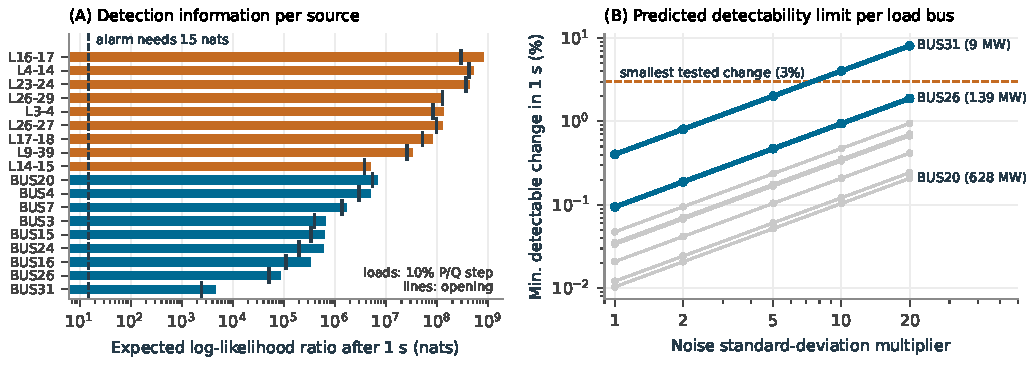
\includegraphics[width=.97\textwidth]{figures/generated/theory_information.pdf}
\caption{Physics-derived detectability from the nominal switched-DAE operators, computed before the attribution campaign. (A) Expected log-likelihood ratio after 1\,s against the no-intervention history (bars) and against the nearest competing source (vertical tick), for a 10\% load step or a line opening; the dashed line marks the evidence $\lambda^\star$ required for an alarm. (B) Minimum load change detectable within 1\,s, \eqref{eq:minimum-detectable}, versus a uniform multiplier of the calibrated noise; gray lines are the other seven load buses.}
\label{fig:theory-information}\end{figure*}

\emph{Prediction 1: detection is not information-limited under the
calibrated noise.} A 10\% load step carries between \RevInfoLoadMin{} and
$\RevInfoLoadMax$ nats in one second, and a line opening at least
$\RevInfoLineMin$ nats, against $\lambda^\star\approx\RevInfoNeed$. The
nearest competitor is separated by a comparable margin, so detection and
isolation should both occur at the first post-onset report and the alarm
should be limited by the six-report confirmation, i.e.\ at about
\RevPredAlarmDelay\,s. Doubling the noise should not change the delay.

\emph{Prediction 2: a single detectability limit.} Under a uniform noise
multiplier, every load except bus~31 remains detectable at the smallest
tested change (3\%) up to a multiplier of~20; the worst of them needs
\RevWorstOtherLoadPctTwenty\% there. The bus-31 load is only
\RevBusThirtyOneMW\,MW, and its 3\% change becomes undetectable within one
second beyond a multiplier of about \RevBusThirtyOneCross.

\emph{Prediction 3: forgetting is costly everywhere.} After every one of
the \RevResetEvents{} interventions of the controlled study, resetting the
physical state gives some birth hypothesis at least
$\RevResetGainMin$ nats of spurious evidence, more than $10^{\RevResetFactorMin}$
times $\lambda^\star$; with carry the spurious evidence is zero.

\emph{Prediction 4: one missing or corrupted PMU does not remove
attribution.} Under independent per-PMU noise of 0.05\% TVE, deleting the
most informative PMU leaves every evaluated intervention at least
\IntInfoMinFactor{} times $\lambda^\star$ in one second (median
\IntInfoMedianFraction\% of the full information retained;
Fig.~\ref{fig:integrity}C). PMU~39 carries the most information about most
sources.

These predictions are deliberately coarse. They use a single linearization,
steady-state covariances and the true onset, and they ignore the proposal
screen and the publication rules. Their value is that they are computed
from the network equations alone and can fail.
